% Claude, generated by tests/plot_som_sweep_iphone.py --average --scenes apple teddy spin paper-windmill block --name iphone_avg
% (branch bd-split-rules): SoM rerun on the current code (seed 42, B = 1..10) averaged over the five iPhone scenes at each B; ours
% (seed 42) at the mean of its per-scene B (apple 5, teddy 8, spin 9, paper-windmill 9, block 7); open circle = SoM averaged at
% each scene's B.
% [Claude] 2026-11-05 (user request): validation only, one panel per dataset, Fig. 2b style, MoMo final (split_init at the tables' B:
% DyCheck 5 8 9 9 10, NVIDIA 4 6 8 7 5 6 6). tests/plot_sweep_val_avg.py -> plots/sweep_val_avg/sweep_val_{dycheck,nvidia}.pdf (copied to img/).
% Seed 42, last epoch, val/fg_psnr. DyCheck SoM sweep: outputs/bdf/som; NVIDIA SoM sweep: the Killarney sweep (outputs/bdf_nvsweep, parity
% with Vulcan within 0.1 dB). Values: DyCheck MoMo 12.64 at B 8.2, SoM at each B 12.64, SoM-10 12.63, SoM peak 12.74 at B 3;
% NVIDIA MoMo 20.42 at B 6.0, SoM at each B 20.19, SoM-10 20.32, SoM max 20.38 at B 9.
\begin{figure}[t]
  \centering
  \begin{subfigure}{\linewidth}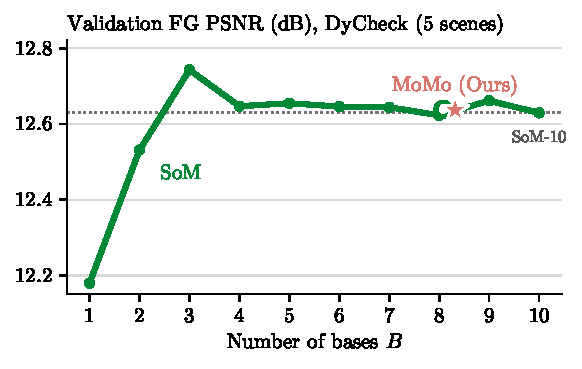
\includegraphics[width=\linewidth]{img/sweep_val_dycheck.pdf}\phantomsubcaption\label{fig:sweep-avg-dycheck}\end{subfigure}\\[2pt]
  \begin{subfigure}{\linewidth}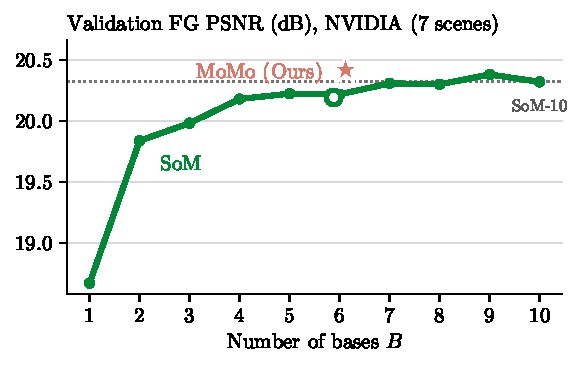
\includegraphics[width=\linewidth]{img/sweep_val_nvidia.pdf}\phantomsubcaption\label{fig:sweep-avg-nvidia}\end{subfigure}
  \caption{\claudetag\ Foreground PSNR on the held-out views against the number of bases, averaged over the five DyCheck
    (iPhone) scenes (top) and the seven NVIDIA scenes (bottom): SoM~\cite{wang2025shape} with $B = 1$--$10$ bases (curve), ours at
    the mean of the $B$ its stopping rule picks per scene (star; 8.2 on DyCheck, 6.0 on NVIDIA) and SoM given each scene's $B$
    (circle); dotted line: SoM-10. Seed 42.}
  \label{fig:sweep-avg}
\end{figure}
